\question{3}{
    Het Korps Mariniers wil onderzoeken of het klimaat waarin mariniers gestationeerd zijn invloed heeft op hun fysieke conditie.
    Hiervoor wordt de conditie voor twee groepen mariniers gemeten via het maximale zuurstofopnamevermogen ($\text{VO}_2\text{max}$, in ml/kg/min).
    De eerste groep is gestationeerd in het noorden van Noorwegen (koud klimaat, populatie $A$) en de tweede groep in Cura\c{c}ao (warm klimaat, populatie $B$).

    \begin{center}
        \begin{tabular}{c|ccccccccc}
            \toprule
                \textbf{$\text{VO}_2\text{max}$ mariniers in koud klimaat} & $62$ & $60$ & $65$ & $64$ & $61$ & $63$ & $66$ & $64$ \\
                \textbf{$\text{VO}_2\text{max}$ mariniers in warm klimaat} & $58$ & $59$ & $57$ & $60$ & $56$ & $58$ & $59$ & $57$ \\
            \bottomrule
        \end{tabular}
    \end{center}
}
    \begin{enumerate}[label=(\alph*)]
        \item Bereken de steekproefgemiddeldes $\overline{x_A}$ en $\overline{x_B}$, en de steekproefvarianties $s_A^2$ en $s_B^2$.
        \answer{
            {\bfseries Populatie $A$: mariniers in koud klimaat.}
            
            We berekenen het steekproefgemiddelde $\overline{x_A}$ als volgt:
            \begin{align*}
                \overline{x_A} = \frac{x_1+x_2+\ldots+x_n}{n} = \frac{ 62 + 60 + \ldots + 64 }{ 8 } = 63,125
            \end{align*}
        

            We berekenen de steekproefvariantie $s_A^2$ als volgt:
            \begin{align*}
                s_A^2   &= \frac{ (x_1 - \overline{x_A})^2 + (x_2 - \overline{x_A})^2 + \ldots + (x_n - \overline{x_A})^2 }{ n - 1 } \\
                        &= \frac{ (62 - 63,125)^2 + (60 - 63,125)^2 + \ldots + (64 - 63,125)^2 }{ 8 - 1 } \\
                        &\approx 4,125.
            \end{align*}
       
            {\bfseries Populatie $B$: mariniers in warm klimaat.}

            We berekenen het steekproefgemiddelde $\overline{x_B}$ als volgt:
            \begin{align*}
                \overline{x_B} = \frac{x_1+x_2+\ldots+x_n}{n} = \frac{ 58 + 59 + \ldots + 57 }{ 8 } = 58
            \end{align*}
        

            We berekenen de steekproefvariantie $s_B^2$ als volgt:
            \begin{align*}
                s_B^2   &= \frac{ (y_1 - \overline{x_B})^2 + (y_2 - \overline{x_B})^2 + \ldots + (y_n - \overline{x_B})^2 }{ m - 1 } \\
                        &= \frac{ (58 - 58)^2 + (59 - 58)^2 + \ldots + (57 - 58)^2 }{ 8 - 1 }\\
                        &\approx 1,7143.
            \end{align*}       
        }

        \item Bepaal met behulp van een $F$-toets of de varianties in $\text{VO}_2\text{max}$ gelijk zijn voor beide groepen mariniers.
            Gebruik het kritieke gebied in je conclusie. 
            Kies voor het significantieniveau $\alpha = 0,05$.
        \answer{
            In de vraag staat dat we aan mogen nemen dat $X_A \sim N(\mu_A=?; \sigma_A=?)$ en $X_B \sim N(\mu_B=?; \sigma_A=?)$.

            We toetsen op gelijke varianties, oftewel de nulhypothese $H_0$ en de alternatieve hypothese $H_1$ worden als volgt gedefinieerd:
            \begin{align*}
                H_0: \quad \sigma_A^2 = \sigma_B^2 \\
                H_1: \quad \sigma_A^2 \neq \sigma_B^2
            \end{align*}

            Verder is gegeven dat we mogen werken met een significantieniveau $\alpha=0,05$, en data is al verzameld voor beide populaties.
            De toetsingsgrootheid voor een $F$-toets is gelijk aan
            \[
                F = \frac{S_A^2}{S_B^2}, 
            \]
            en volgt een $F(n-1, m-1)$-verdeling, oftewel een $F(13, 16)$-verdeling.

            De geobserveerde toetsingsgrootheid is gelijk aan
            \[
                f = \frac{s_A^2}{s_B^2} = \frac{4,125}{1,7143} \approx 2,4062.
            \]
            
            Omdat we tweezijdig toetsen, is het kritieke gebied van de vorm $(-\infty; g_1]$ en $[g_2; \infty)$, waarbij de grenzen $g_1$ en $g_2$ bepaald kunnen worden met de $F(5,9)$-verdeling.
            \begin{align*}
                &\fcdf(\text{lower}=0; \text{upper}=g_1; \text{df1}=7; \text{df2}=7)=\alpha/2=0,025 \rightarrow g_1 \approx 0,2002\\
                &\fcdf(\text{lower}=g_2; \text{upper}=10^{99}; \text{df1}=7; \text{df2}=7)=\alpha/2=0,025 \rightarrow g_2 \approx 4,9949
            \end{align*}
            De berekende $f = 2,4062$ ligt dus niet in het kritieke gebied, dus we mogen de nulhypothese $H_0$ accepteren.
            Er is op basis van deze steekproeven onvoldoende bewijs om de aanname van gelijke varianties te verwerpen.
            We mogen dus uitgaan van gelijke varianties en de gemeenschappelijke $\sigma = \sigma_A = \sigma_B$ schatten aan de hand van de ``pooled variance''.

            \begin{center}
                \resizebox{0.9\textwidth}{!}{
                    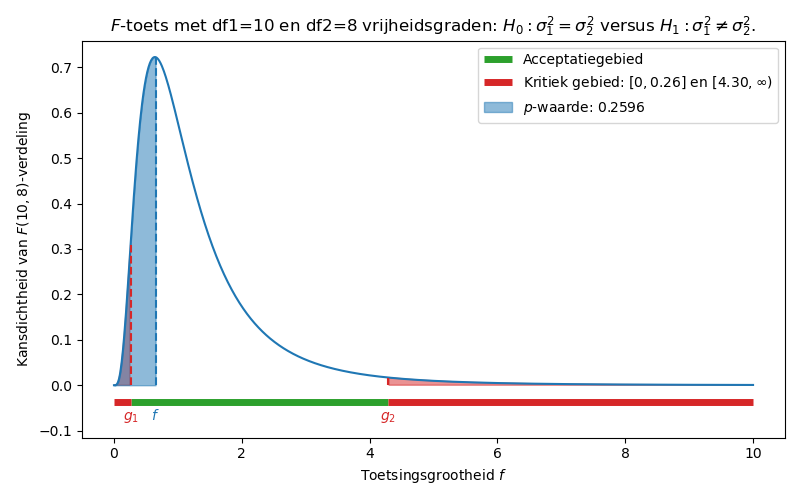
\includegraphics{oefenopgave3_Ftoets.png}
                }
            \end{center}
        }

        \item Bepaal met behulp van een onafhankelijke $t$-toets of de gemiddelde $\text{VO}_2\text{max}$-waardes significant van elkaar afwijken
        voor beide groepen mariniers.
            Formuleer een conclusie op basis van de $p$-waarde.
            Kies opnieuw voor het significantieniveau $\alpha = 0,05$.
        \answer{
            We toetsen of de gemiddelde $\text{VO}_2\text{max}$-waardes $\mu_B$ voor de populaties mariniers in respectievelijk koude en warme klimaten significant van elkaar afwijken.
            De hypotheses kunnen we daarom als volgt defini\"eren:
            \begin{align*}
                H_0: \quad \mu_A = \mu_B \text{ (geen significant afwijking) } \\
                H_1: \quad \mu_A \neq \mu_B \text{ (wel een significante afwijking) }
            \end{align*}

            Verder is gegeven dat we mogen werken met een significantieniveau $\alpha=0,05$, en data is al verzameld voor beide populaties.

            Op basis van ons antwoord bij vraag (b) mogen we aannemen dat $\sigma = \sigma_A = \sigma_B$.
            Dat betekent dat we met de pooled variance mogen werken als schatting voor de gemeenschappelijke onbekende $\sigma$.
            
            \begin{align*}
                s_P^2 = \frac{(n-1)\cdot s_A^2 + (m-1) \cdot s_B^2}{n-1+m-1} = \frac{7 \cdot 4,125 + 7 \cdot 1,7143}{14} \approx 2,9196.
            \end{align*}
            
            De toetsingsgrootheid van de bijbehorende $t$-toets is (onder de nulhypothese $\mu_A = \mu_B$) gelijk aan
            \begin{align*}
                t &= \frac{(\overline{x_A}-\overline{x_B}) - (\mu_A - \mu_B)}{\sqrt{\frac{s_P^2}{n} + \frac{s_P^2}{m}}} \\
                  &= \frac{(63,125 - 58) - 0}{\sqrt{\frac{2,9196}{9} + \frac{2,9196}{9}}} \\
                  &\approx 5,9987. 
            \end{align*}

            en komt uit een $t$-verdeling met $\text{df}=n+m-2 = 8 + 8 - 2 = 14$ vrijheidsgraden.
            Omdat we tweezijdig toetsen, is de $p$-waarde gelijk aan de rechteroverschrijdingskans van de waarde $t \approx 5,9987$ (deze is kleiner dan de linkeroverschrijdingskans omdat de $t$-verdeling symmetrisch rond $0$ is), oftewel
            \begin{align*}
                p = P(T \ge t) = \text{tcdf}(\text{lower}=5,9987; \text{upper}=10^{99}; \text{df}=13) \approx 1,6310 \cdot 10^{-5}.
            \end{align*}
            
            Omdat de $p$-waarde (veel) kleiner is dan het significantieniveau $\alpha = 0,05$, moet de nulhypothese $H_0$ worden verworpen.
            Er is op basis van deze steekproeven voldoende reden om aan te nemen dat de gemiddelde $\text{VO}_2\text{max}$-waardes van mariniers die in respectievelijk koude en warme klimaten gestationeerd zijn, significant van elkaar afwijken.
            \begin{center}
                \resizebox{0.9\textwidth}{!}{
                    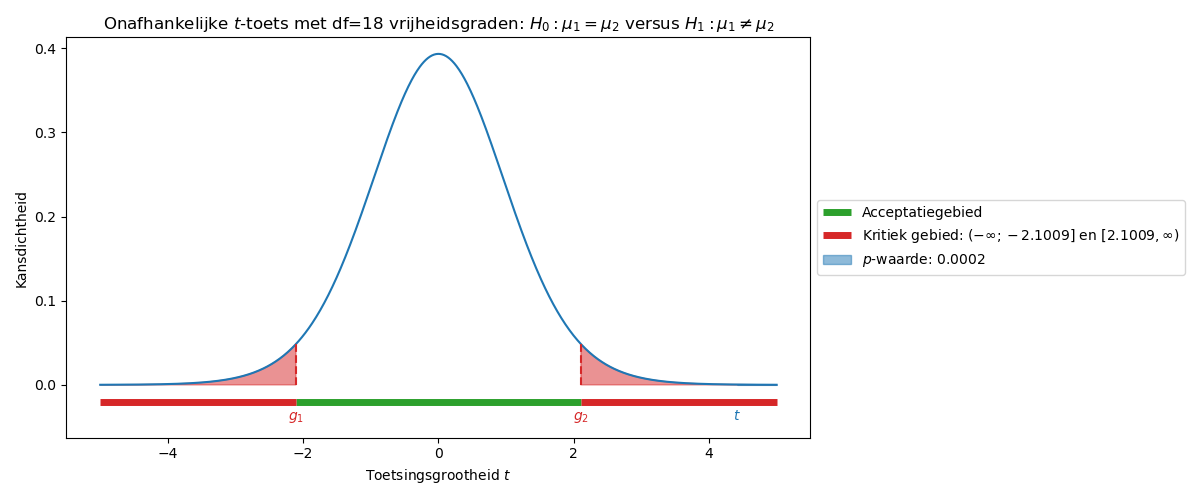
\includegraphics{oefenopgave3_ttoets.png}
                }
            \end{center}

            {\itshape Side note: bij dit soort vragen is het interessant om te kijken wat de toetsuitslag ons nu eigenlijk zegt en hoe dat te verklaren is.
            De toetsuitslag geeft aan dat er een significante afwijking is, maar niet de richting.
            Uit de data is echter op te maken dat de $\text{VO}_2\text{max}$-waardes vrijwel consistent hoger liggen voor de mariniers in het koude klimaat.
            Wellicht heeft dit te maken met het feit dat in koude klimaten minder zuurstof in de lucht zit.
            Het lichaam moet dan zelf harder werken en meer rode bloedlichaampjes produceren om genoeg zuurstof binnen te krijgen, waardoor de zuurstofopname verbeterd wordt.}
        }    
    
    \end{enumerate}